% design and analysis
%
% DESIGN AND ANALYSIS: Objective of the study, data source, statistical model/tools/methodology, 
% validity of the assumptions if any, results of the study (graphs, tables will go here),
% results discussion, (interpretations/consclusions/inferences)
%
%----------------------------------------------------------------------------------------
%	PACKAGES AND OTHER DOCUMENT CONFIGURATIONS
%----------------------------------------------------------------------------------------
%

\section{Design and Analysis}
To best model the dichotomous response variable, Y\textunderscore HighGradeCancer, in the Prostate Cancer case study, I will employ a multiple logistic regression model, where 1 indicates high grade cancer and 0 indicates not high grade cancer. \par

In statistics, if \(\pi = f(x)\) is a probability then \(\frac{\pi}{1-\pi}\) is the corresponding \textit{odds}, and the \textbf{logit} of the probability is the logarithm of the odds:
\begin{equation}
	logit(\pi) = log(\frac{\pi}{1-\pi})
\end{equation}


Now, simple logistic regression means assuming that \(\pi(x)\) is related to \(\beta_0 + \beta_1x\) (the \textit{logit response function}) by the logit function. By equating \(logit(\pi)\) to the logit response function (Eqn. X), we understand that the logarithm of the odds is a linear function of the predictor. In particular, the slope parameter \(\beta_1\) is the change in the log odds associated with a one-unit increase in x. This implies that the odds itself changes by the multiplicative factor \(e^{\beta_1}\) when x increases by 1 unit.

\begin{equation}
	log(\frac{\pi}{1-\pi}) = \beta_0 + \beta_1x
\end{equation}

From here, straightforward algebra will then show the Simple Linear Regression Model:

\begin{equation}
	E[Y] = \pi(x) = \frac{e^{\beta_0 + \beta_1x}}{1+e^{\beta_0 + \beta_1x}}
\end{equation}

 \par

Next, this simple logistic regression model is easily extended to more than one predictor variable by inclusion of the following two vectors, in matrix notation:

\[
	\boldsymbol{\beta} = 
	\begin{bmatrix}
		\beta_0 \\ \beta_1 \\ \vdots \\ \beta_{p-1}
	\end{bmatrix} \quad
	\textbf{X} = 
	\begin{bmatrix}
		1 \\ X_1 \\ X_2 \\ \vdots \\ X_{p-1}
	\end{bmatrix} 
\]

% might need to reference this column vector at a later time
%	\textbf{X}_i =
%	\begin{bmatrix}
%		1 \\ X_{i1} \\ X_{i2} \\ \vdots \\ X_{i,p-1}
%	\end{bmatrix}

With this notation, the simple logistic response function (1) extends to the multiple logistic response function as follows:

\begin{equation}
	E[Y] = \pi(\textbf{X}) = \frac{exp(\textbf{X}'\boldsymbol{\beta})}{1+exp(\textbf{X}'\boldsymbol{\beta})}
\end{equation}

Fitting the logistic regression to the sample data requires that the parameters \(\beta_0\), \(\beta_1\), \(\cdots\), \(\beta_{p-1}\) be estimated. This will be done using the maximum likelihood technique provided within the statistical packages of both \textbf{R} and Python.


\subsection{Data Transformations and Standardization}
In modeling using logistic regression, the appropriate transformations on continuous variables are necessary to optimize the model predictiveness. \par
Variable transformation is an important technique to create robust models using logistic regression. Because the predictors are linear in the log of the odds, it is often helpful to transform the continuous variables to create a more linear relationship. \par
The raw data collected contained several predictors with high skewness values.
A few concerning features were determined to be PSA Level (skewness = 4.39), Cancer Volume (skewness = 2.18), and Weight (skewness = 7.46). As a prepossessing step to reduce skewness, I elected to transform these continuous predictor variables using the log-transformation, and standardize \textit{all} the data on top of that. The standardization step was used to normalize the data, did not affect any underlying distributions, and was performed by using the following design: \par 

The finalized data skewness is summarized directly below. Following, I've included the histogram of PSA Level vs. Cancer Volume vs. Age, a helpful visual for the three predictors which carried the most significance through much of my analysis.


\begin{figure}[H]
	\centering
	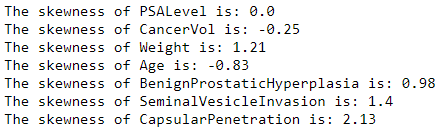
\includegraphics{final_SKEWNESS.png}
	\caption{insert caption here.}
\end{figure}


\begin{figure}[H]
	\centering
	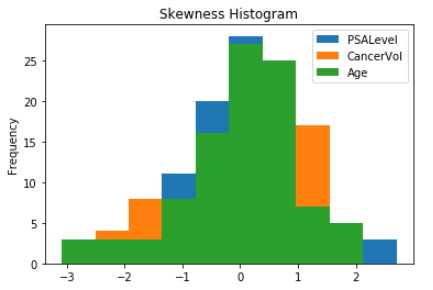
\includegraphics{psa_cancervol_age_SKEWNESS.png}
	\caption{insert caption here.}
\end{figure}

\subsection{Second-Order Predictors}
Occasionally, the first-order logistic model may not provide an adequate fit to the data, so I began my analysis by first attempting to fit the Prostate Cancer data to a \textit{polynomial logistic} regression model. For simplicity, a 2\textsuperscript{nd}-order polynomial model in two predictors has a logit response function as

\begin{equation}
logit(\pi) = \beta_0 + \beta_1x_1 + \beta_2x_2 + \beta_{11}x_1^2 + \beta_{22}x_2^2 + \beta_{12}x_1x_2
\end{equation}

\noindent and can be extended to more predictors by the inclusion of additional variables, their coefficients, and accompanying cross terms. Please recall, the Prostate Cancer data set considers 7 predictors.
% $\boldsymbol{\beta}$ and \textbf{X}, as I described previously in \S 4.1.


In many situations the true regression function XXX has one or more peaks or valleys, and in such cases a polynomial function can provide a satisfactory approximation to XXX. However, a polynomial fit was not successful here, as indicated by \textit{non-significant} p-values across all predictors, at 5\% significance. Additionally, my preliminary scatter plot analysis did not indicate any reason to believe a polynomial fit would be suitable in this study. Without hesitation, I will move forward with the development of a multiple logistic \textit{linear} regression model.

\begin{figure}[H]
	\centering
	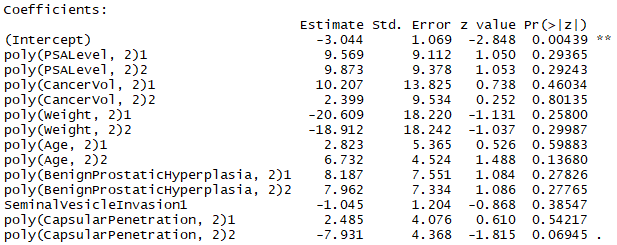
\includegraphics[scale=0.9]{poly_output}
	\caption{insert caption here}
\end{figure}





\subsection{Model Selection}

\subsubsection{Best Subsets Procedure}
The procedure outlined here will help identify a group of subset models that give the best values of a specified criterion. This technique has been developed by time-saving algorithms which can find the most promising models, without having to evaluate all \(2^{p-1}\) candidates. The use of the best subset procedure is based on the \textit{AIC\textsubscript{p}} criteria, where promising models will yield a relatively small value. \par

The minimized \textit{AIC\textsubscript{p}} stepwise output given by \textbf{R} is provided in Figure XXX below.

\begin{figure}[H]
	\centering
	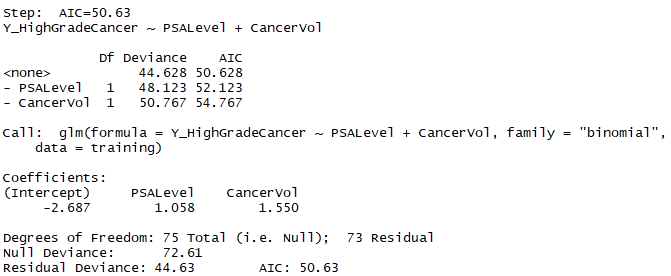
\includegraphics[scale=0.9]{best_subset}
	\caption{insert my caption here}
\end{figure}

In this procedure, I instructed \textbf{R} to iterate "backwards" through all 7 predictor variables and it was determined \textit{AIC\textsubscript{p}} was minimized for \(p=3\). In particular, the results reveal that the best two-predictor model for this criteria is based on PSA Level and Cancer Volume.


\subsubsection{Final Model}
The data of 97 individual men in the Prostate Cancer sample was split at 80\% for train and test sets. The training set is a random 76 observations and was used for fitting the model, and the remaining 21 cases were saved to serve as a validation data set. Table XXX in columns 1-X contains the variables... The primary purpose of the study was to asses the strength of the association between each of the predictor variables, the predictable nature of PSA Level, and the probability of a man having been diagnosed with high grade prostate cancer over low grade. \par

A first-order multiple logistic regression model with two predictor variables was considered to be reasonable by \S4.3: 

\begin{equation}
\pi(\textbf{X}) = \frac{exp('\boldsymbol{\beta})}{1+exp(\textbf{X}'\boldsymbol{\beta})} = [1+exp(-\textbf{X}'\boldsymbol{\beta})]^{-1}
\end{equation}

where:

\begin{equation}
\textbf{X}'\boldsymbol{\beta} = \beta_0+\beta_1X_1+\beta_2X_2
\end{equation}

This model was fitted by the method of maximum likelihood to the data from the 76 train cases. The results are summarized in Table XXX below. The estimated logistic response function is:

\begin{equation}
\hat{\pi}=[ 1+ exp(-2.6867 + 1.0577X_1 + 1.5502X_2)]^{-1}
\end{equation}

%%% MAYBE I SHOULD INCLUDE THIS IN THE CONCLUSION INSTEAD
Now, the interpretation for multiple logistic regression is that the estimated odds ratio for the predictor variable \(X_k\) assumes that all other predictor variables are held constant. We can see, for instance, that the odds of a man being diagnosed with high grade prostate cancer increase by about 105\% for each additional score of PSA Level, for a given Cancer Volume. This means each unit increase of PSA Level approximately doubles the odds of said diagnosis. 

\subsubsection{Geometric Interpretation}
When fitting a standard multiple logistic regression model with two predictors, the estimated regression shape is an S-shaped surface in three-dimensional space. Figure XXX displays a three-dimensional plot of a logistic response function that depicts the relationship between the diagnosis of high grade prostate cancer (\textit{Y}, the binary outcome) and two continuous predictors, PSA Level (\textit{X}\textsubscript{1}) and Cancer Volume (\textit{X}\textsubscript{2}). This surface increases in an approximately linear fashion for larger values of PSA Level and Cancer Volume, but levels off and is nearly horizontal for small values of these predictors.

With the estimated logistic regression equation now developed, it is left to analyze the residuals, test goodness of fit, and finally apply the model to the test data and discuss the results.

\subsection{Analysis of Residuals}

\subsubsection{Logistic Regression Residuals}
\subsubsection{Influential Observations}

\subsection{Goodness Of Fit Evaluation}
The appropriateness of the fitted logistic regression model needs to be examined before it is accepted for use. In particular, we need to examine whether the estimated response function for the data is monotonic and sigmoidal in shape, as are logistic response functions. Here I will employ the Hosmer-Lemeshow test, which is useful for unreplicated data sets, as is the Prostate Cancer data. The test can detect major departures from a logistic response function, and the alternatives of interest are as follows:

\begin{align}
\begin{split}
	H_0: E[Y]=  [1+exp(-\textbf{X}'\boldsymbol{\beta})]^{-1} \\
	H_0: E[Y] \neq  [1+exp(-\textbf{X}'\boldsymbol{\beta})]^{-1}
\end{split}
\end{align}

\subsubsection{Hosmer-Lemeshow}
The Hosmer-Lemeshow Goodness of Fit procedure consists of grouping that data into classes with similar fitted values \(\hat{\pi}_i\), with approximately the same number of cases in each class. Once the groups are formed, the Hosmer-Lemeshow goodness of fit statistic is calculated by using the Pearson chi-square test statistic of observed and expected frequencies. The test statistic is known to be well approximated by the chi-square distribution with \(c-2\) degrees of freedom.

\begin{equation}
	\chi^2 = \sum_{j=1}^{c} \sum_{k=0}^{1} \frac{(O_{jk}-E_{jk})^2}{E_{jk}}
\end{equation}

The output from \textbf{R} using 5 groups is shown in Figure XXX.

\begin{figure}[H]
	\centering
	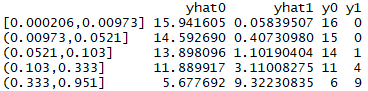
\includegraphics{gof_detail}
	% \caption{insert caption here}
	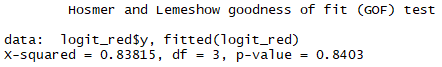
\includegraphics{gof_results}
	\caption{caption here}
\end{figure}

Large values of the test statistic X\textsuperscript{2} indicate that the logistic response function is not appropriate. The decision rule for testing the alternatives in (Eqn. XXX), when controlling the level of significance at \(\alpha\), therefore is:

\begin{align}
\begin{split}
	\textrm{If X\textsuperscript{2}} \leq \chi^2(1-\alpha; c-p)\textrm{, conclude } H_0 \\
	\textrm{If X\textsuperscript{2}} > \chi^2(1-\alpha; c-p)\textrm{, conclude } H_a
\end{split}
\end{align}

Thus, for \(\alpha=0.5\) and \(c-2=3\), we require \(\chi^2(.95; 3)=7.81\). Since \(X^2=0.838\leq7.81\), we conclude \textit{H}\textsubscript{0}, that the logistic response function is appropriate. The \textit{p}-value of the test is 0.8403.

\subsection{Development of ROC Curve}
Multiple logistic regression is often employed for making predictions for new observations.
The \textit{receiver operating characteristic} (ROC) \textit{curve} plots \(P(\hat{Y}=1 | Y=1)\) as a function of \(1-P(\hat{Y}=0 | Y=0)\) is an effective way to graphically display prediction rule information, and possible cutoff points. \par

The "True Positive" y-axis on an ROC curve is also known as \textit{sensitivity}, and the "False Positive" x-axis is 1-\textit{specificity}. Figure XXX below exhibits the ROC curve for model XXX for all possible cut points between 0 and 1.

\begin{figure}[H]
	\centering
	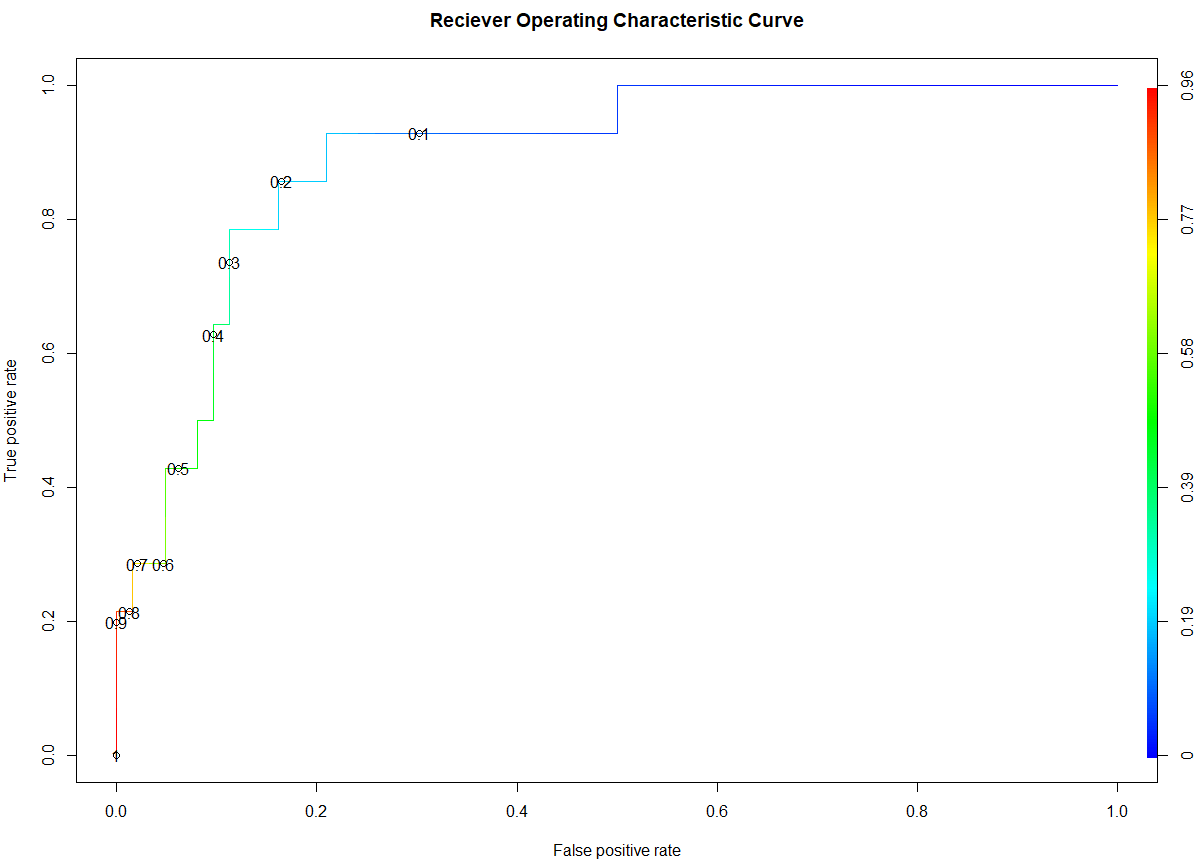
\includegraphics[scale=0.4]{roc_v2}
	\caption{insert caption here}
\end{figure}

\subsubsection{Prediction Rule}
In the training data set (which represented a random 80\% of the 97 provided observations), there were 14 men who were observed as high grade cancer patients; hence the estimated proportion of persons who had high grade cancer is \(14/76=0.184\). This proportion can be used as the starting point in the search for the best cutoff in the prediction rule. \par

Thus, if \(\hat{\pi}_h\) represents a newly fitted observation, my first prediction rule investigated was:
\begin{equation}
	\textrm{Predict 1 if } \hat{\pi}_h \geq 0.184\textrm{; predict 0 if } \hat{\pi}_h < 0.184
\end{equation}

Table XXX below provides a summary of the number of correct and incorrect classifications based on prediction rule XXX. Of the 62 men without high grade cancer, 13 would be incorrectly predicted to have high grade cancer, or an error rate of 21.0\%. Furthermore, of the 14 persons with high grade cancer, 1 would be incorrectly predicted with rule XXX to not have it, or 7.1\%. Altogether, \(13+1=14\) of the 76 predictions would be incorrect, so that the prediction error rate for rule XXX is \(14/76=0.184\) or 18.4\%. Coincidentally, the model exactly matches our training set proportions with the current prediction rule. \par


\begin{table}[H]
	\centering
	\begin{tabular}{ |c||c|c||c|  }
 	\hline
 	\multicolumn{4}{|c|}{Prediction Rule XXX} \\
 	\hline\hline
 	True Classification&\(\hat{Y}=0\)&\(\hat{Y}=1\)&Total\\
 	\hline
 	\(Y=0\)&49&13&62\\
 	\(Y=1\)&1&13&14\\
 	\hline\hline
 	Total&50&26&76\\
 	\hline
	\end{tabular}
 	\caption{Classification based on Logistic Response Function XXX and Prediction Rules.}
\end{table}

With this baseline understood, it is straightforward to choose a stronger cutoff point in utilizing the ROC curve of Figure XXX. As detailed above, the false-positive rate is not ideal at 21.0\%; there are too many cases where a man may opt for additional screening and treatment, even invasive actions, because he believes he has prostate cancer. It will be wise to now reference the ROC curve to better choose a prediction cutoff, while also not significantly disturbing the false-negative accuracy. \par

Looking at Figure XXX I see a step occurring at 0.20, and use this value for my cutoff candidate. The effects of this change can be summarized in the Confusion Matrix table below. \\
The model accuracy has now increased with a significantly better false-negative rate, thus intended to reduce the footprint across the health care economy. \par

Thus, my updated and final prediction rule is stated as follows:
\begin{equation}
	\textrm{Predict 1 if } \hat{\pi}_h \geq 0.2\textrm{; predict 0 if } \hat{\pi}_h < 0.2
\end{equation}

\subsection{Model: Strengths and Weaknesses}

\subsubsection{Strengths}
\subsubsection{Weaknesses}
-gof has less than 5 expected frequencies 
-psa level and cancer volume correlations